\documentclass[9pt,twocolumn,twoside]{gsajnl}
% Use the documentclass option 'lineno' to view line numbers
\usepackage{booktabs}
\usepackage{siunitx}
\usepackage{adjustbox}
\usepackage{geometry} % just not to bother with the table width
%\usepackage[colorinlistoftodos]{todonotes} % comments in margins
%\setlength{\marginparwidth}{1.25cm}
%\definecolor{flame}{rgb}{0.89, 0.35, 0.13}
%\newcommand{\josh}[1]{\textcolor{flame}{\emph{\scriptsize {#1}}}}
%\newcommand{\citex}{\textcolor{red}{\bf (CITE)\,}}
%\newcommand{\out}[1]{\textcolor{red}{#1}} %outline placeholder text
\newcommand{\X}{\textcolor{red}{\bf X\,}}

\articletype{gos} % article type
% {inv} Investigation
% {gs} Genomic Selection
% {goi} Genetics of Immunity
% {gos} Genetics of Sex
% {mp} Multiparental Populations

\title{Reduced Nucleotide Diversity on a Plant Y Chromosome Following Recent Recombination Suppression}

\author[$\ast$,$\dagger$,1]{Josh Hough}
\author[$\dagger$]{Wei Wang}
\author[$\dagger$]{Spencer C.H. Barrett}
\author[$\dagger$]{Stephen I. Wright}

\affil[$\ast$]{Department of Plant Sciences, University of California, Davis}
\affil[$\dagger$]{Department of Ecology and Evolutionary Biology, University of Toronto}

%\affil[$\dagger$]{Author two affiliation}
%\affil[$\ddagger$]{Author three affiliation}
%\affil[$\S$]{Author four affiliation}
%\affil[$\ast\ast$]{Author five affiliation}

\keywords{Sex Chromosome Evolution; Nucleotide Diversity; Recombination; Deleterious Mutations}

\runningtitle{Plant sex chromosome evolution} % For use in the footer

\correspondingauthor{Josh Hough}

\begin{abstract}
X and Y chromosomes differ in effective population size ($N_{e}$), rates of recombination, and exposure to natural selection, all of which can significantly affect levels of genetic variability within the genome. On Y chromosomes with suppressed recombination, both positive and negative selection can remove genetically linked neutral variation, resulting in a reduction in $N_{e}$ and the level of polymorphism on Y compared to X chromosomes or autosomes. However, non-selective factors including female biased sex ratios and high variance in male fitness can also reduce Y-linked $N_{e}$, making it difficult infer the causes of low Y-chromosome diversity. Here, we investigate the factors affecting X- and Y-linked polymorphism during the early stages of plant sex chromosome evolution in \textit{Rumex hastatulus} (Polygonaceae). Strikingly, we find that nucleotide diversity on the Y chromosome is 40 fold lower than on the X chromosome. We demonstrate that the magnitude of this reduction is not consistent with a purely neutral model based on the occurrence of female biased sex ratios in this species, or by reduced male $N_{e}$ caused by high variance in male fitness. Rather, using forward simulations, we show that the diversity reduction on the Y is consistent with the predicted effects of purifying selection removing deleterious mutations and linked neutral variation. Given the recent origin of \textit{R. hastatulus} sex chromosomes, our results indicate that the low level of sequence diversity commonly observed on ancient Y chromosomes can evolve soon after sex chromosomes originate, with background selection playing an important role during the early stages of their evolution.
\end{abstract}

\setboolean{displaycopyright}{true}

\begin{document}

\maketitle
\thispagestyle{firststyle}
\marginmark
\firstpagefootnote
\correspondingauthoraffiliation{jhough@ucdavis.edu}
\vspace{-11pt}

\section*{Introduction}

\lettrine[lines=2]{\color{color2}M}{}orphologically distinct sex chromosomes have evolved multiple times independently in both plant and animal kingdoms \citep{westergaard1958,ohno1967,bull1983,charlesworth1991}. Despite numerous biological differences between the kingdoms, X and Y chromosomes in both lineages have undergone similar genetic changes, suggesting that general evolutionary mechanisms might drive sex chromosome divergence \citep{charlesworth1978,charlesworth1996CB,charlesworth2000degeneration}. Investigating the shared features of plant and animal sex chromosomes, including the loss of recombination \citep{bergero2009}, the degeneration of Y chromosomes \citep{hough2014,bergero2015}, and the evolution of dosage compensation \citep{muyle2012,papadopulos2015}, thus provides an informative context for investigating the evolutionary forces driving sex chromosome evolution.

One fundamental difference between sex chromosomes and autosomes is their respective copy number in a population; whereas autosomes in diploid species are present in two copies in each sex, the X chromosome is present in two copies in females and only one copy in males. As a consequence, the effective population size ($N_{e}$) of the X chromosome is predicted to be 3/4 that of autosomes, whereas the $N_{e}$ of the male-limited Y chromosome is expected to equal 1/4 that of autosomes (assuming an equal number of reproducing females and males). Such differences in $N_{e}$ are predicted to directly affect relative levels of neutral polymorphism maintained on these chromosomes, which is proportional to the product of $N_{e}$ and the neutral mutation rate, $\mu$ \citep{Kimura1984}. This variation in neutral polymorphism is in turn expected to have important consequences on patterns of DNA sequence evolution, including the effectiveness of both positive and negative selection \citep{charlesworth1987}.

Several demographic factors can modulate or accentuate differences in polymorphism levels maintained on sex chromosomes \citep{ellegren2009}. These include population subdivision and sex-biased dispersal, deviations from a 1:1 breeding sex ratio, and high variance in reproductive success \citep{caballero1995,charlesworth2001,laporte2002,pool2007}. For example, studies comparing levels of variability on the X chromosome and autosomes in humans have found evidence that sex-biased dispersal has reduced levels of X-to-autosome diversity below the neutrally expected level of 0.75 \citep{keinan2009}, though there is considerable variation in estimates of the X/A ratio in humans, and other demographic processes have also been suggested \citep{hammer2010,bustamante2009}. Theoretical work also indicates that population bottlenecks can lead to disproportionate decreases in sex-linked compared to autosomal variation \citep{pool2007}, a prediction that has been supported in a diverse array of taxa, including chimpanzees and orangutans \citep{kaessmann2001,fischer2006}, the house mouse \textit{Mus musculus} \citep{baines2007}, Drosophila \citep{andolfatto2001}, and humans \citep{keinan2009}.

In addition to demographic factors, evolutionary theory predicts that genetic variability on sex chromosomes should be affected by the evolution of suppressed X-Y recombination, which lowers the coalescent $N_{e}$ for Y-linked genes and increases their vulnerability to the effects of selective sweeps \citep{smith1974hitch,aquadro1994} and background selection \citep{charlesworth1996background,charlesworth1994effect}. These processes can be viewed as examples of the Hill–Robertson (HR) effect, in which the effective population size for a given chromosomal region depends strongly on the rate of recombination, such that selection at a focal site is not independent of selection at nearby sites \citep{hill1966HReffect}. Moreover, both background selection and selective sweeps predict a reduction in $N_{e}$ and, as a result, reduced levels of neutral polymorphism, selection efficacy, and rate of adaptation \citep{comeron2008}. Although the HR effect can occur throughout the genome \citep{mcvean2000}, large genomic regions in which recombination is suppressed, such as the Y chromosome, are expected to experience the most severe reductions in neutral diversity due to chromosome-wide linkage \citep{charlesworth1996CB,charlesworth2000degeneration,bachtrog2013NRG}. Consistent with this, studies examining Y chromosome variability in mammals \citep{hellborg2004,Wilsonsayres2014} and Drosophila \citep{mcallister1999,bachtrog2000} have found that Y-linked diversity is considerably lower than predicted under models of neutral evolution, suggesting that the HR effect plays a key role determining patterns of nucleotide diversity during sex chromosome evolution across a broad range of animal taxa.

Despite widespread interest in determining the effects of recombination on patterns of genetic diversity \citep{ellegren2011,bachtrog2013NRG}, we still know very little about the influence of the HR effect on patterns nucleotide polymorphism in younger sex chromosome systems, where \textit{de novo} recombination suppression evolved relatively recently \citep{charlesworth2016plant}. Recent studies of young plant sex chromosome systems have revealed that several canonical features of X and Y chromosome evolution are shared between plants and animals, including the genetic deterioration of the Y chromosome \citep{bergero2015,hough2014}, the occurrence of ‘evolutionary strata’ \citep{bergero2009}, and the evolution of dosage compensation \citep{muyle2012,papadopulos2015}. Nonetheless, except for a small number of genes in \textit{Silene latifolia} \citep{filatov2001diversity,qiu2010nucleotide}, the associated changes in genetic diversity that are predicted from evolutionary models of X- and Y-chromosome evolution have not been widely studied in plant sex chromosomes. Given that background selection and selective sweeps are predicted to have the strongest effects during the earliest stages of Y-chromosome evolution, before Y-chromosomes have lost the majority of their genes \citep{bachtrog2008temporal}, studying recently evolved sex chromosomes provides an important test of the temporal dynamics of the HR effect.

To investigate the factors affecting nucleotide diversity in the early stages of sex chromosome evolution, we analyzed single nucleotide polymorphisms (SNPs) on sex chromosomes and autosomes in the plant \textit{R. hastatulus }(Polygonaceae). This species is a dioecious annual with highly heteromorphic X and Y chromosomes that are estimated to have evolved  approximately 15 MYA \citep{quesada2011,grabowska2015,navajas2005}, making sex chromosomes in this species over 100 million years younger than the well-studied mammalian sex chromosomes \citep{lahn1999,ross2005dna}. \textit{Rumex hastatulus} has also received particular attention because of the unique occurrence of an intraspecific sex chromosome system, in which both XY and $XY_{1}XY_{2}$ males occur in geographically distinct 'chromosomal races' \citep{smith1963mechanism}. The $XY_{1}XY_{2}$ sex chromosome system in this species (the North Carolina race) is thought to have originated through an X-autosome fusion, with the XY system (the Texas race) maintaining the ancestral chromosome complement \citep{smith1964evolving}. Despite the recent origin of sex chromosomes in both races, a recent study revealed that both the ancestral and neo-Y chromosomes have undergone significant genetic degeneration\citep{hough2014}.

Of particular relevance to the present study, \textit{R. hastatulus} populations have also been found to consistently exhibit female-biased sex ratios, with a mean sex ratio of $N_{m}/N_{f}=0.6$ \citep{pickup2013influence}. This is important because female-biased sex ratios are predicted to affect chromosomal $N_{e}$ and therefor the level of genetic diversity maintained on sex chromosomes and autosomes \citep{ellegren2009}. Here, we investigated whether the patterns of diversity we observed on sex chromosomes and autosomes were jointly consistent with predictions from models of sex ratio bias and variance in reproductive success, or whether linked selection (background selection and selective sweeps) has played a greater role.

\section*{Materials and Methods}
\subsection*{Population Samples and Sex-Linked Genes}
We analyzed sex-linked and autosomal genes identified from Illumina RNA sequence data from 24 individuals (12 males and 12 females, with 1 male and 1 female from each of 12 populations; 6 populations of each sex chromosome race). Samples were collected in 2010 from throughout the native range of \textit{R. hastatulus} (locations in Table S1), and plants were grown in the glasshouse from seeds collected from open-pollinated females. We extracted RNA from leaf tissue using Spectrum Plant Total RNA kits (Sigma-Aldrich). The isolation of mRNA and cDNA synthesis was conducted according to standard Illumina RNAseq procedures, with sequencing conducted on two Illumina HiSeq lanes with 150-bp end reads at the Genome Quebec Innovation Center. Reads from these 24 samples were mapped to the \textit{R. hastatulus} reference transcriptome \citep{hough2014}, and raw sequences are available from the Gen-Bank Short Read Archive under accession no. SRP041588. Reads were mapped using the Burrows–Wheeler Aligner \citep{li2010fast}, followed by Stampy \citep{lunter2011stampy}. We used Picard tools (http://picard.sourceforge.net) to modify mapping output into the format required for the Genome Analysis Toolkit \citep{mckenna2010genome} variant calling software, and subsequently removed genes with low coverage (<10x) and Phred Quality Scores <20. The population samples analyzed here were previously reported in Hough et al. (2014), where they were used to validate the ascertainment of sex-linked genes identified through segregation analysis. Here, we focused on the set of 460 sex-linked genes for which the Y homolog was inferred to be on the $y_{1}$ chromosome (i.e., sex-linked genes that are shared between the Texas and North Carolina races).

\subsection*{Autosomal Genes}
In evaluating evidence for nucleotide diversity differences between X and Y chromosomes, it is important to distinguish between reduced Y-linked diversity, and the possibility that X-linked diversity is elevated above the level predicted from a neutral model. To do this, we normalized sex-linked diversity estimates by autosomal diversity, and compared empirical X/A and Y/A nucleotide diversity ratios to those predicted from a neutral model (described below). Because the criteria for identifying autosomal loci in Hough et al. (2014) were based on the occurrence of four segregating SNPs per locus, this set of genes is probably higher in diversity than the average autosome. Therefore, for the present analysis we incorporated the broader set of all non-sex linked (punitively autosomal) genes from our transcriptome data. We also filtered this set to remove genes that may have been sex-linked but were not identified as such by the conservative ascertainment criteria in Hough et al. (2014). In particular, we removed: (i) any genes in which there was evidence for at least one SNP with a sex-linked segregation pattern, (ii) any genes with SNPs showing fixed heterozygosity in males and fixed homozygosity in females, (iii) any genes with less than 10X coverage or greater than 100X coverage from independently obtained genomic coverage data (to filter out duplicate genes or those with highly repetitive sequences), and (iv) any genes containing SNPs with large (>0.4) allele frequency differences between males and females. Finally, we removed genes with fewer than 100 synonymous sites following this filtering to avoid biasing our results toward genes that may have been particularly short due to assembly problems. This filtering resulted in a set of 12,356 and 11,350 autosomal genes in the Texas and North Carolina races, respectively.

\subsection*{Phasing X and Y alleles}
To estimate polymorphism for the X and Y sequences separately, it is necessary to infer the phase of SNPs in sex-linked transcripts in males. In previous work, phasing alleles on \textit{R. hastatulus} sex chromosomes was achieved using segregation analysis from a genetic cross. Here, to phase SNPs from population samples where such segregation data was unavailable, we used HAPCUT \citep{bansal2008hapcut}, a maximum-cut based algorithm that reconstructs haplotypes using sequenced fragments (Illumina read data) from the two homologous chromosomes to output a list of phased haplotype blocks containing the SNP variants on each chromosome. Because the resulting haplotype blocks produced by HAPCUT contained SNPs that were phased relative to each other, but not designated to either the X or Y chromosome, we assigned individual variants to X or Y by independently identifying fixed X-Y differences with each haplotype block (i.e., sites in which all females were homozygous, and all males were heterozygous). Identifying such fixed differences within phased haplotype blocks enabled us to then infer the correct phase (X or Y) of the polymorphisms from HAPCUT’s output. This was done by matching the phase of fixed X-Y differences with their neighboring polymorphic sites - i.e., when a fixed X-Y difference occurred in the same phased haplotype block as a polymorphic site, the polymorphic variants in that block were assigned to either X or Y based on the known phase of the fixed difference with which they were matched. SNPs that were identified outside of phased blocks, or in blocks without fixed X-Y differences, were recorded as missing data. Finally, we filtered out SNPs with coverage > 60, QUAL score > 60, and those within a distance of 10bp or less from indels. This procedure was conducted using a combination of Perl and Bash scripts, and resulted in fasta-formatted alignments of X and Y sequences for 372 sex-linked genes from the 24 individuals in our study.

We further validated the results of HAPCUT’s allele phasing by comparing the accuracy of this method with the phasing-by-segregation method that was conducted using data from a genetic cross in Hough et al. (2014). To do this, we first phased the sequence data from parents and their progeny using HAPCUT’s algorithm (using the same parameters as for the population data). In particular, we looked for cases where SNPs were inferred on the Y chromosome by HAPCUT, but where the ‘true’ level polymorphism was inferred to be zero by phasing-by-segregation. We identified 7 percent of sex-linked genes with phasing errors of this kind, or that were determined to have genotyping errors resulting in a false SNP calls on the Y chromosome, with a SNP error rate estimate of 1.7 x 10-4. This rate is very low relative to the population-based estimates of polymorphism on the X and autosomes (Table 1), and therefore should have minimal effects on our estimation of X/A polymorphism. However, because this rate is high relative to the expected level of true polymorphism on the Y-chromosome, we further filtered genes in which we found evidence for false-positive Y-polymorphisms arising from: (i) phasing errors caused by gene duplicates (more than two haplotypes), (ii) polymorphisms around indels, and (iii) genotyping errors caused by low Y-expression. This filtering was done by manually inspecting sequences in IGV \citep{robinson2011integrative} and identifying each individual putative polymorphism on the Y chromosome.

\subsection*{Estimating nucleotide diversity on sex chromosomes and autosomes}
For each locus in our analysis, we calculated Watterson’s (1975) estimator of the population parameter $\theta=4N_{e}\mu$, where $N_{e}$ is the effective population size, and $\mu$ is the mutation rate \citep{watterson1975}, using a modified version of the Perl program Polymorphurama \citep{bachtrog2006}. To compare sex-linked and autosomal loci, we calculated the average value of $\theta$, weighted by the number of synonymous sites in each gene (\X Figure 2; Table 1). We obtained 95 percent confidence intervals for our estimates of the X/A and Y/A diversity ratios by bootstrapping by gene using the BCa method \citep{efron1994} implemented in the Boot package in R \citep{canty2012boot}, and calculating X/A and Y/A diversity on each iteration for 20000 replicates each. Bootstrapping was conducted on the final filtered set of 173 sex-linked, and 12355 autosomal genes from the Texas race, and separately for the 176 sex-linked and 11349 autosomal genes from the North Carolina race. Note that the lack of recombination on the Y chromosome implies that assumptions of independent loci are likely violated such that the true uncertainty in our Y/A diversity estimate obtained by this method is likely underestimated. To address this issue, we used a maximum likelihood approach, implemented a modified version of the MLHKA software \citep{wright2004hka}, to independently estimate a credibility interval for the Y/A ratio (Figure S1). We also tested whether estimates of diversity for the X chromosome calculated from phased sequences from females were consistent with estimates from phased sequences from males. As no significant difference was observed (\X Figure? Table?), we report only results from females.

Finally, we tested for population substructure between the two sex chromosome races to control for the possibility that hidden substructure in our sampled populations could affect estimates of diversity. To do this, we conducted a phylogenetic analysis of sex-linked sequences from all populations in our study. The analysis was conducted on an alignment of X- and Y-linked genes from \textit{R. hastatulus}, with orthologous autosomal sequences from the non-dioecious but closely related outgroup species \textit{R. bucephalophorus} used to root the tree (Figure S2). The phylogeny was inferred using the Neighbor-Joining method \citep{saitou1987neighbor}, with evolutionary distances computed using Maximum Composite Likelihood \citep{tamura2011mega5}. The inferred sequence phylogeny revealed strong support for Y-linked genes from the $XY_{1}XY_{2}$ ("North Carolina") race being paraphyletic (98 percent bootstrap support), with samples from two populations (hereafter the SC sub-clade) forming a monophyletic group, and samples from Florida and Georgia (hereafter the FL sub-clade) also forming a monophyletic group, but more closely related to the XY (Texas) race (Figure S2). In light of this evidence for population substructure, we used the inferred phylogeny as the basis for estimating X and Y diversity.  

\subsection*{Neutral predictions and the effect of sex ratio bias on diversity}
To test whether the levels of diversity we observed on X, Y and autosomal chromosomes could be explained by the occurrence of biased reproductive sex ratios or high variance in reproductive success, we compared our empirical estimates of diversity to predictions from a neutral model that jointly considers these two effects. Here, following Nomura (2002), the effective population sizes for autosomal loci is given by:

\begin{equation}
N_{e{A}} = \frac{4N_{m}N_{f}}{N_{m}(1+C^2_{f})+N_{f}(1+C^2_{m})}\label{eq:NeA}
\end{equation}

where $N_{m}$ and $N_{f}$ are effective population sizes for males and females, respectively, and $C^2_{i}$ is the coefficient of variation in mating success for the $i$th sex, defined as the ratio of the standard deviation to the mean number of mates $\sigma_{i}/\mu_{d{i}}$. Similarly, for X and Y linked loci, 

\begin{equation}
N_{e{X}} = \frac{9N_{m}N_{f}}{4N_{m}(1+C^2_{f})+2N_{f}(1+C^2_{m})}\label{eq:NeX}
\end{equation}

and

\begin{equation}
N_{e{Y}} = \frac{N_{m}(1+C^2_{f})}{2}\label{eq:NeY}
\end{equation}

With with no variation in mating success in either sex ($C^2_{m}=C^2_{f}=0$), equations 1-3 reduce to the familiar expressions from \citep{wright1931evolution}:

\begin{equation}
N_{e{A}} = \frac{4N_{m}N_{f}}{N_{m}+N_{f}}\label{eq:NeA}
\end{equation}


\begin{equation}
N_{e{X}} = \frac{9N_{m}N_{f}}{4N_{m}+2N_{f}}\label{eq:NeX}
\end{equation}

\begin{equation}
N_{e{Y}} = \frac{N_{m}}{2}\label{eq:NeY}
\end{equation}

To consider the joint effects of biased sex ratios and variance in male reproductive success, our neutrally-expected levels of diversity were calculated using equations 1-3, assuming no variance in female mating (e.g., $C^2_{f}=0$), and we considered a range of values for $\sigma_{m}$: 0 (no variance), 1/2 (Poisson/2) 1 (Poisson distribution of offspring), 2 (Poisson*2), and 3 (Poisson*3). Figure 1 shows the predicted effective population size of autosomes and sex chromosomes as a function of the sex ratio and variance in male reproductive success. Using these neutral predictions, we compared our empirically estimated diversity levels to normalized X/A and Y/A ratios of diversity, assuming that the level of neutral polymorphism is given by the product of the mutation rate and the effective population size, $\theta=4N_{e}\mu$ \citep{watterson1975,kimura1984}. Note that we have only considered variance in male reproductive success here because this is most likely to occur in wind pollinated plant like \textit{R. hastatulus}, where males produce copious amounts of pollen and compete to fertilize uniovulate females (\X ref).


%old stuff
%The effect of biased reproductive sex ratios on the $N_{e}$ for an autosomal gene can be estimated using the equation \citep{wright1931evolution}:

%\begin{equation}
%N_{e} = \frac{4N_{m}N_{f}}{N_{m}+N_{f}}\label{eq:Ne}
%\end{equation}

%where $N_{m}$ and $N_{f}$ are the numbers of reproducing males and females, respectively. Similarly, for an X-linked gene, where females contain two-thirds and males one-third of the alleles, the effective population size is given by:  

%\begin{equation}
%N_{e{X}} = \frac{9N_{m}N_{f}}{4N_{m}+2N_{f}}\label{eq:NeX}
%\end{equation}

%And, for the male-limited Y chromosome: 

%\begin{equation}
%N_{e{Y}} = \frac{N_{m}}{2}\label{eq:NeY}
%\end{equation}


%\begin{equation}
%\frac{N_{e_{X}}}{N_{e_{A}}} = \frac{9(N_{f}+N_{m})}{8(2N_{f}+N_{m})}\label{eq:X/A}
%\end{equation}

%and, 

%\begin{equation}
%\frac{N_{e_{Y}}}{N_{e_{A}}} = \frac{9(N_{f}+N_{m})}{8(2N_{f}+N_{m})}\label{eq:X/A}
%\end{equation}


 %Given a female effective population size $N_{f}$, and a male effective population size $N_{m}$, the predicted effective population size for X-linked genes, relative to autosomes, is given by $N_{e_{X}}/N_{e_{A}} = 9(N_{f}+N_{m})/8(2N_{f}+N_{m})$ (Wright 1931). Similarly, for the Y chromosome, the effective population size is given by 1/4 the total $N_{e}$ or 1/2 the $N_{e}$ of males, $N_{m}$/2. Thus, with equal sex ratios, $N_{e_{X}}/N_{e_{A}} = 0.75$, and $N_{e_{Y}}/N_{e_{A}} = 0.25$. For populations with female-biased sex ratios, however, $N_{m}$ becomes small relative to $N_{f}$ and this ratio can become larger than 1, approaching 1.125 at the limit \citep{caballero1995}. With the level of nucleotide polymorphism maintained in a population is proportional to the product of the mutation rate and the effective population size: $\theta=4N_{e}\mu$ \citep{watterson1975,kimura1984}. Figure 1 shows the predicted effective population size ratios for autosomal, X-linked, and Y-linked genes (left) and the corresponding X/A and Y/A ratios of diversity (right) for a sex ratio bias ranging from $N_{f}/(N_{f}+N_{m})=0$ to $N_{f}/(N_{f}+N_{m})=1$.

%In particular, Wright's (1931) formula $N_{e}=4N_{f}N_{m}/(N_{f} + N_{m})$ gives the effective population size of a randomly mating population with separate sexes and a Poisson distribution of offspring number. For a female effective population size $N_{f}$, and a male effective population size $N_{m}$, the predicted effective population size for X-linked genes relative to autosomes is given by $N_{e_{X}}/N_{e_{A}} = 9(N_{f}+N_{m})/8(2N_{f}+N_{m})$ (Wright 1931). With equal sex ratios, $N_{e_{X}}/N_{e_{A}} = 0.75$. For populations with female-biased sex ratios, however, $N_{m}$ becomes small relative to $N_{f}$ and this ratio can become larger than 1, approaching 1.125 at the limit \citep{caballero1995}. For the Y chromosome, the effective population size is given by 1/4 the total $N_{e}$ or 1/2 the $N_{e}$ of males, $N_{m}$/2. Under neutrality, the level of nucleotide polymorphism maintained in a population is proportional to the product of the mutation rate and the effective population size: $\theta=4N_{e}\mu$ \citep{watterson1975,kimura1984}. Assuming equal neutral mutation rates for all genes and an equal number of reproducing males and females, Y-linked genes should therefore have 1/3 the polymorphism of X-linked genes, and 1/4 that of autosomal genes. Figure 1 shows the predicted effective population size ratios for autosomal, X-linked, and Y-linked genes (left) and the corresponding X/A and Y/A ratios of diversity (right) for a sex ratio bias ranging from $N_{f}/(N_{f}+N_{m})=0$ to $N_{f}/(N_{f}+N_{m})=1$.

\begin{figure}[htbp]
\centering
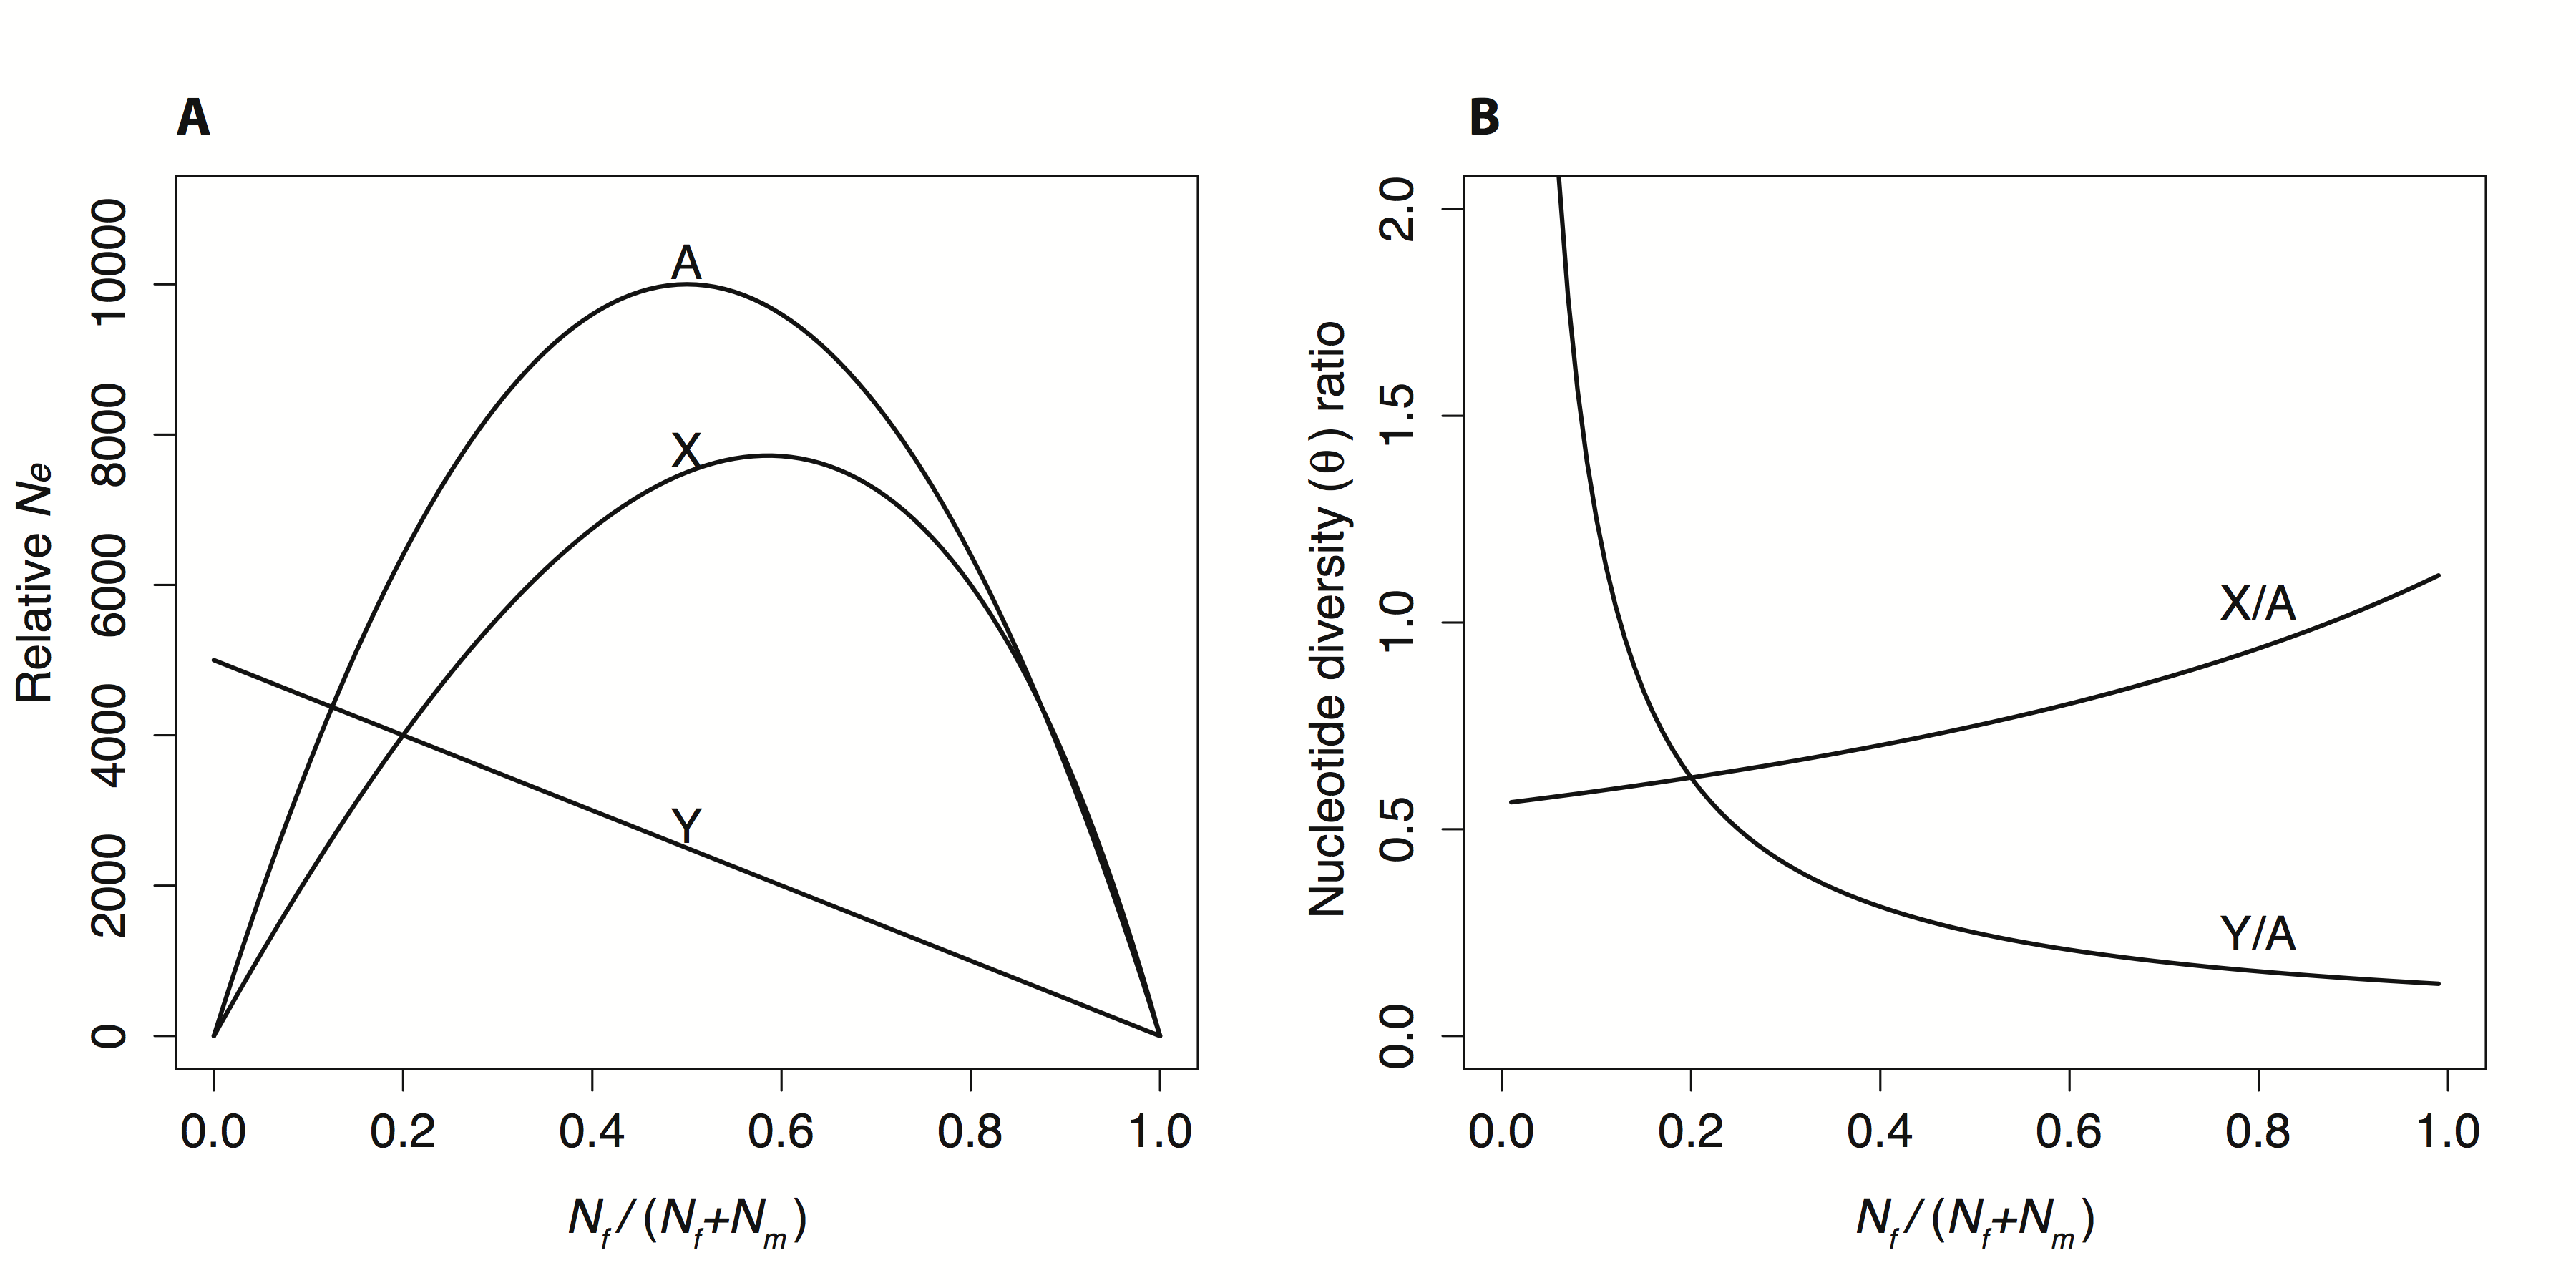
\includegraphics[width=\linewidth]{Figure1.png}
\caption{The relation between relative effective population size and sex ratio bias for genes on autosomes (\textbf{A}) and sex chromosomes (\textbf{B}) (Y chromosome in red). The sex ratio is shown as the proportion of males, $N_{m}/(N_{f}+N_{m})$, where $N_{m}$ and $N_{f}$ are the effective number of breeding males and females, respectively, plotted against $N_{e}/N$, where $N=N_{m}+N_{f}$ and the $N_{e}$ for sex chromosomes and autosomes is given in equations 1-3. Dotted curves show predictions in the standard neutral model, where both males and females produce Poisson-distributed offspring numbers and the chromosomal $N_{e}$'s are given by equations 4-6 \citep{wright1931evolution}. Solid curves correspond to increasing levels of variance in male reproductive success \citep{nomura2002effective} (see Methods). Assuming $\theta=4N_{e}\mu$ and equal neutral mutation rates among genes, the predicted $N_{e}$'s are used to generate null predictions for X/A and Y/A ratios of diversity.  
}%
\label{fig:spectrum}
\end{figure}

\subsection*{Simulations of positive and purifying selection}
To test whether our observed level of Y-chromosome diversity could be explained by selection, we conducted two sets of forward-time simulations using the software SFSCODE \citep{hernandez2008flexible}: (i) Purifying selection acting to remove deleterious mutations and linked neutral variation (i.e., background selection), and (ii) Positive selection acting on beneficial mutations and reducing variation through selective sweeps (refs \X). For purifying selection simulations, we assumed that selection coefficients followed a gamma distribution, and we considered a range of values for the mean selection coefficient ($s$) by varying the scale parameter, $k$ (range \X) from (\X) to \X and keeping the shape parameter, \X, constant (see Supporting Information for simulation code). To make the simulation output comparable to our data, we initialized simulations with our empirically estimated value of $\theta$ (estimated from autosomes), and sampled 8 chromosomes per simulation from 24 populations. For simulating positive selection, we used \X [parameters here]. We ran 1000 replicates for each model and calculated the average $\theta_{sim}$ and the corresponding Y/A ratio of neutral diversity under the both sets of models separately. We then tested the significant of the fit of our simulated diversity output to our empirical data (\X new figure) by calculating the proportion of simulation replicates for which $\theta_{sim}$ was not significantly different from $\theta_{observed}$, using a two-sided P value. Commands for running the simulations are provided in the Supporting Information. 

\section*{Results and Discussion}

\subsection*{Y-chromosome diversity in \textit{R. hastatulus} is very low}
Our analysis revealed that diversity on the \textit{R. hastatulus} Y chromosome is significantly lower than expected under neutrality, with estimates indicating Y/A=0.02, which is 12.5 fold lower than the standard neutral prediction of Y/A = 0.25 (P<0.0001), and 40-fold lower compared to mean diversity on the X chromosome (Table 1). Note that by normalizing X and Y diversity by autosomal diversity, our results indicate that the X-Y difference we observed was not due to an elevation of X chromosome diversity, but rather a Y-specific reduction. Conceivably, such low diversity on the Y could arise from a low mutation rate on the Y chromosome, or a lower mutation rate in males compared to females. However, these possibilities can be rejected because there is no evidence that the number of synonymous mutations in X and Y lineages, estimated by both parsimony and maximum likelihood, are significantly different \citep{hough2014}. 

It is worth noting that our results only apply to the $Y_{1}$ chromosome as estimates of diversity were calculated for sex-linked genes that were shared between the $XX/XY$ and the $XX/XY_{1}Y_{2}$ sex chromosome systems. Previous work found that both the $Y_{1}$ and the more recently evolved "neo" $Y_{2}$ chromosomes exhibited signs of genetic degeneration, including gene loss, loss of expression, and an accumulation of amino acid-changing mutations \citep{hough2014}, but we cannot say from the present study whether the neo-Y chromosome has also undergone a reduction in diversity. However, the extensive reduction in diversity estimated on the $Y_{1}$ chromosome occurs in each of the three \textit{R. hastatulus} sub-clades (\X Figure 2; Table 1; Figure S2), suggesting that this effect is not population-specific.

\begin{table}[t!]
\centering
\caption{Estimates of neutral diversity by race on \textit{R. hastatulus} sex chromosomes and autosomes.}
\begin{tabular}{ccccccccc}
\textbf{} & \multicolumn{2}{c}{\textbf{Texas}} & \multicolumn{2}{c}{\textbf{South Carolina}} & \multicolumn{2}{c}{\textbf{Florida}} \\
chromosome & $\theta$ & $\theta/\theta_{A}$ & $\theta$ & $\theta/\theta_{A}$ & $\theta$ & $\theta/\theta_{A}$ \\
\midrule
A & 0.006 & 1 & 0.006 & 1 & 0.005 & 1 \\    
X & 0.0047 & 0.85 & 0.002 & 0.33 & 0.0047 & 0.37 \\ 
Y & $\num{e-4}$ & 0.002 & $\num{e-4}$ & 0.002 & $\num{e-4}$ & 0.002 \\ 
\addlinespace

\bottomrule
\end{tabular}
\end{table}

Although our sampling of each \textit{R. hastatulus} sub-clade is limited, the discovery of three phylogenetically distinct monophyletic groups is interesting because it suggests the possibility that introgression occurred between the ancestral Texas (XY race) and the derived North Carolina ($XY_{1}Y_{2}$) race, leading to a derived $XY_{1}Y_{2}$ sub-clade. As the North Carolina and Texas races are known to be inter-fertile \citep{smith1964evolving}, we suggest that the SC sub-clade inferred here likely originated through hybridization between a female from the FL clade harboring the X-autosome fusion, and a male from the XY Texas race. Notably, when we pooled the samples from each sub-clade together, the estimated level of Y diversity was significantly higher in the pooled data, highlighting the presence of strong substructure between these groups (Figure S2).

Our results also indicate a significant reduction in X/A diversity in the derived SC and FL sub-clades of the North Carolina race ($X/A_{FL}=0.33$ and $X/A_{SC}=0.37$) compared to the Texas race ($X/A_{TX}=0.85$) (Figure 2). Although not expected, this reduction in diversity may be associated with the recent origin of the $XY_{1}Y_{2}$ sex chromosome system, which is thought to have originated through an X-autosome fusion involving the ancestral 3rd chromosome in the Texas race \citep{smith1964evolving}. Evidence supporting this autosomal origin was recently obtained by \citep{grabowska2015}, who reported that the ancestral third chromosome in the Texas race carries the 5S rDNA locus, which is now found on both the neo-X and the $Y_{2}$ sex chromosomes in the derived North Carolina race. If recent positive selection was involved in driving the evolution of this X-A fusion, which theory suggests as likely \citep{charlesworth1980sex}, then the formerly autosomal segment on the X chromosome in the $XY_{1}Y_{2}$ sub-clades may have experienced a strong selective sweep, resulting in reduced X-linked diversity in the derived $XY_{1}Y_{2}$ sub-clades. It will be important for future work to investigate in more detail the factors driving the establishment of the X-autosome fusion in this species, and how they might impact patterns of X-linked neutral diversity. 

In contrast to the situation on the X chromosome, our data indicate a strong and consistent diversity reduction on the Y chromosome, and we now consider several models that might explain this reduction.

\subsection*{Female biased sex ratio and high variance in male fitness}

 A highly reduced level of Y chromosome variability is a predicted outcome of models Y-chromosome evolution based on the removal of deleterious mutations and linked neutral variants (e.g., background selection), but the occurrence of female-biased sex ratios in this species has also been predicted to lower Y diversity in the absence of such selective interference (\X ref). Moreover, reduced Y-linked diversity could be accented by high variance in male reproductive success (Figure 1). This is not unusual in annual plants such as \textit{R. hastatulus}, which commonly exhibit extensive phenotypic plasticity in plant size and flower production (\X Harper 1977). Conceivably, such plastic differences among plants, owing to spatial heterogeneity in resources, could influence the intensity of male-male competition, and thus affect variance in male reproductive success. Given that male plants in this wind-pollinated species produce large amounts of pollen, and that female flowers are uniovulate, strong competition among males is expected. 
 
 In common with most flowering plants we do not have marker-based estimates of the variance in male reproductive success in \textit{R. hastatulus}. However, by comparing our empirical estimates of diversity to predictions from models that jointly predict the effects on diversity of sex ratio bias and male reproductive variance, we evaluated whether these effects could explain the level of Y/A diversity that we observed (see Methods). Conditioning on estimates of sex ratio bias in \textit{R. hastatulus} that have been estimated, ranging from $N_{m}/(N_{m}+N_{f})=0.4$ to $N_{m}/(N_{m}+N_{f})=0.35$ \citep{pickup2013influence}, the predicted Y/A diversity ratio  under a Poisson distribution of offspring numbers, is approximately 0.2 (Table1, Figure 3). Our estimated mean Y/A ratio, however, is 0.02, which is significantly lower ($\textit{P}<0.0001$), suggesting that the sex ratio effect alone is insufficient to explain our data. For larger values for the variance in male reproductive success (\X) given this sex ratio, the corresponding predictions for Y/A are all significantly higher than our observed ratio (\X table). 
 Finally, neutral models that could not be rejected, i.e., in which a highly female-biased sex ratio (\X) and a high variance in male reproductive success predict a Y/A ratio that fit out data (\X), can be excluded because they simultaneously predicted X/A ratios that were significantly different from what we observed (\X Figure). Thus, our results indicate that the combined effects of sex ratio bias and variance in reproductive success cannot jointly explain our observed levels of X, Y, and autosomal diversity in \textit{R. hastatulus}.
 
\subsection*{Background Selection and Selective Sweeps}

\section*{Conclusions}

\section*{Acknowledgments}


\bibliography{bibliography}
\end{document}
